\documentclass[a4paper, 12pt]{article}
\usepackage{comment} % enables the use of multi-line comments (\ifx \fi) 
\usepackage{lipsum} %This package just generates Lorem Ipsum filler text. 
\usepackage{fullpage} % changes the margin
\usepackage[a4paper, total={7in, 10in}]{geometry}
\usepackage{amsmath}
\usepackage[russian, english]{babel}
\usepackage[utf8]{inputenc}
\usepackage[T2A]{fontenc}
\usepackage{amssymb}  
\usepackage{graphicx}
\newcommand{\squeeze}{}

%%%%%%%

%%% for coloring rows in a table
%\usepackage[flushleft]{threeparttable}
\usepackage{threeparttable}


\usepackage{multirow}
\usepackage{colortbl}
\definecolor{bgcolor}{rgb}{0.8,1,1}
\definecolor{bgcolor2}{rgb}{0.8,1,0.8}

%%%%%%%%
\usepackage{graphicx} %Loading the package
\graphicspath{{../Experiments/}}

\newcommand{\eqdef}{\; { := }\;}
\newcommand{\R}{\mathbb{R}}
\newcommand{\N}{\mathbb{N}}
\newcommand{\Ind}{\mathbb{I}}
\newcommand{\Exp}{\mathbb{E}}
\newcommand{\ExpBr}[1]{\mathbb{E}\left[#1\right]}
\newcommand{\Cases}[1]{\begin{cases}#1\end{cases}}
\newcommand{\norm}[1]{\left\|#1\right\|}
\def\<#1,#2>{\langle #1,#2\rangle}
\newcommand{\cX}{\mathcal{X}}
\newcommand{\bJ}{\mathbf{J}}
\newcommand{\dom}{\operatorname{dom}}
\newcommand{\prox}{\operatorname{prox}}
\newcommand{\footeq}[1]{{\footnotesize #1}}
\newcommand{\newalpha}{h}
\usepackage{tcolorbox}
\usepackage{pifont}
\definecolor{mydarkgreen}{RGB}{39,130,67}
\definecolor{mydarkred}{RGB}{192,47,25}
\newcommand{\green}{\color{mydarkgreen}}
\newcommand{\red}{\color{mydarkred}}
\newcommand{\cmark}{\green\ding{51}}%
\newcommand{\xmark}{\red\ding{55}}%

\newcommand{\mA}{\mathbf{A}}
\newcommand{\mB}{\mathbf{B}}
\newcommand{\mC}{\mathbf{C}}
\newcommand{\mH}{\mathbf{H}}
\newcommand{\mI}{\mathbf{I}}
\newcommand{\mU}{\mathbf{U}}
\newcommand{\mZ}{\mathbf{Z}}

\newcommand{\cC}{{\mathcal{C}}}
\newcommand{\cH}{{\mathcal{H}}}
\newcommand{\cW}{{\mathcal{W}}}
\newcommand{\cQ}{{\mathcal{Q}}}

\usepackage{amsmath,amsfonts,amssymb,amsthm,array}


\usepackage{mdframed} 
\usepackage{thmtools}
\usepackage{textcomp}

%\theoremstyle{shaded}
\declaretheorem[within=section]{definition}
\declaretheorem[sibling=definition]{theorem}
\declaretheorem[sibling=definition]{proposition}
\declaretheorem[sibling=definition]{assumption}
\declaretheorem[sibling=definition]{corollary}
\declaretheorem[sibling=definition]{conjecture}
\declaretheorem[sibling=definition]{lemma}
\declaretheorem[sibling=definition]{example}
\declaretheorem[sibling=definition]{remark}

%\usepackage[russian]{babel}
\renewcommand{\proofname}{Proof}
% TO DO NOTES 
\usepackage[colorinlistoftodos,bordercolor=orange,backgroundcolor=orange!20,linecolor=orange,textsize=scriptsize]{todonotes}



\usepackage{microtype}
\usepackage{subfigure}
\usepackage{booktabs} % for professional tables


\usepackage{grffile}


\usepackage{hyperref}

\newcommand{\theHalgorithm}{\arabic{algorithm}}
\setlength{\marginparwidth }{2cm} 
\begin{document}
	\noindent{\bf Fundamental theorems of machine learning}  
	\hfill{\bf Islamov Rustem}
	\rule{7in}{1.8pt}\\
	
	\section{Problem}
	
	\begin{figure}[h]
	\begin{center}
	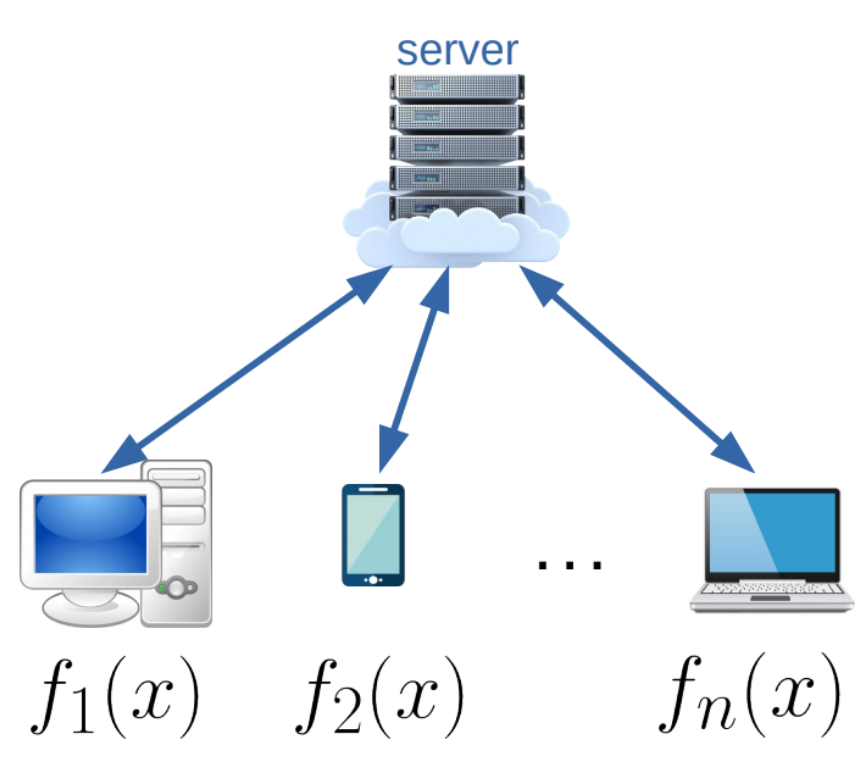
\includegraphics[width=0.4\linewidth]{plots/1.png}
	\end{center}
	\caption{Model of centralized distributed framework.}
	\end{figure}
	
	\noindent We consider L2 regularized empirical risk minimization problems of the form
\begin{equation}\label{primal}
\squeeze 
\min \limits_{x\in \mathbb{R}^d} \left[ P(x) \eqdef f(x) + \frac{\lambda}{2}\|x\|^2  \right],
\end{equation}
where $f:\R^d \to \R$ is a smooth\footnote{Function $\phi:\R^d\to \R$ is {\em smooth} if it is differentiable, and has $L_\phi$ Lipschitz gradient: $\|\nabla \phi(x)- \nabla \phi(y)\| \leq L_\phi  \|x-y\|$ for all $x,y\in \R^d$. We say that $L_\phi$ is the {\em smoothness constant} of $\phi$.} convex function of the ``average of averages'' structure
\begin{equation} \label{eq:f_and_f_i} 
 \squeeze f(x) \eqdef\frac{1}{n}\sum \limits_{i=1}^n  f_i(x), \quad f_i(x) \eqdef \frac{1}{m} \sum \limits \limits_{j=1}^{m} f_{ij}(x), \end{equation}
and $\lambda\geq 0$ is a regularization parameter. Here $n$ is the number of parallel workers (nodes), and $m$ is the number of training examples handled by each node\footnote{All our results can be extended in a straightforward way to the more general case when node $i$ contains $m_i$ training examples. We decided to present the results in the special case $m=m_i$ for all $i$ in order to simplify the notation. }.  
The value $f_{ij}(x)$ denotes the loss of the model parameterized by vector $x\in \R^d$ on the $j^{\rm th}$ example owned by the $i^{\rm th}$ node. This example is denoted as $a_{ij} \in \R^d$, and the corresponding loss function is $\varphi_{ij}:\R \to \R$, and hence we have
\begin{equation}\label{eq:f_ij} f_{ij}(x) \eqdef \varphi_{ij}(a_{ij}^\top x).\end{equation}

\noindent Thus, $f$ represents the average loss/risk over all $nm$ training datapoints, and problem \eqref{primal} seeks to find the model whose (L2 regularized) empirical risk is minimized. We make the following assumption. 
\begin{assumption}\label{as:general}
Problem (\ref{primal}) has at least one optimal solution $x^*$. For all  $i$ and $j$, the loss function $\varphi_{ij}: \mathbb{R} \to \mathbb{R}$ is twice differentiable, and its second derivative $\varphi_{ij}^{\prime\prime} : \R \to \R$ is $\nu$-Lipschitz continuous.
\end{assumption} 

\noindent Note that in view of \eqref{eq:f_ij}, the Hessian of $f_{ij}$ at point $x$ is
\begin{equation}
\label{eq:87ybfd0fd}
\mH_{ij}(x) \eqdef 
\nabla^2 f_{ij}(x) = 
\newalpha_{ij}(x) a_{ij}a_{ij}^\top, 
\end{equation}
where
\begin{equation}\label{eq:h_ij-def} \newalpha_{ij}(x) \eqdef \varphi^{\prime\prime}_{ij}(a_{ij}^\top x).\end{equation} In view of Assumption~\ref{as:general}, we have $|\varphi''_{ij}(t)| \leq \gamma$ for all $t\in \R$, and 
\begin{equation}
|\newalpha_{ij}(x) - \newalpha_{ij}(y)| \leq \nu |a_{ij}^\top x - a_{ij}^\top y| \leq \nu \|a_{ij}\|  \|x-y\| \label{eq:alphaijL} 
\end{equation}
for all $x, y \in \R^d$. Let $R\eqdef \max_{ij} \|a_{ij}\|$. The Hessian of $f_i$ is given by
\begin{equation}\label{eq:H_i} \squeeze \mH_i(x) \overset{\eqref{eq:f_and_f_i}  }{=}
%\nabla^2 f_i(x)  
\frac{1}{m}\sum\limits_{j=1}^m \mH_{ij}(x) \overset{\eqref{eq:87ybfd0fd}}{=} \frac{1}{m}\sum\limits\limits_{j=1}^m \newalpha_{ij}(x) a_{ij}a_{ij}^\top,\end{equation}
and the Hessian of $f$ is given by
\begin{equation}\label{eq:H}\squeeze \mH(x) \overset{\eqref{eq:f_and_f_i}  }{=}
%\nabla^2 f_i(x)  
\frac{1}{n}\sum\limits_{i=1}^n \mH_{i}(x) \overset{\eqref{eq:H_i}}{=} \frac{1}{nm}\sum \limits_{i=1}^n   \sum\limits_{j=1}^m \newalpha_{ij}(x) a_{ij}a_{ij}^\top.\end{equation}

\section{{\sf NEWTON-STAR}: Newton's method with a single Hessian} \label{subsec:Newton-star}

We now introduce a simple idea which, surprisingly, enables us to {\em remove the need to iteratively communicate any coefficients altogether.}  Assume, for the sake of argument, that we know the values  $\newalpha_{ij}(x^*)$ for all $i,j$. That is, assume the server has access to coefficients $\newalpha_{ij}(x^*)$ for all $i,j$, and that each node $i$ has access to coefficients $\newalpha_{ij}(x^*)$  for $j=1,\dots,m$, i.e., to the vector
\begin{equation}\label{eq:8f0d8hfd}\newalpha_{i}(x) \eqdef (\newalpha_{i1}(x),\dots, \newalpha_{im}(x)) \in \R^m\end{equation}
for $x=x^*$.  Next, consider the following new Newton-like method which we call {\sf NEWTON-STAR (NS)}, where the ``star'' points to the method's reliance on the knowledge of the optimal solution $x^*$:
\begin{eqnarray}  x^{k+1} &=& x^k - \left(\nabla^2 P(x^*) \right)^{-1} \nabla P(x^k) 
\overset{\eqref{primal}}{=} x^k - \left(\mH(x^*) +\lambda \mI \right)^{-1} \left(\frac{1}{n}\sum_{i=1}^n \nabla f_i(x^k) + \lambda x^k\right).\label{eq:Newton-star}\end{eqnarray}

\noindent Since the server knows $\mH(x^*)$, all that the nodes need to communicate are the local gradients $\nabla f_i(x^k)$, which costs $O(d)$ per node. The server then computes $x^{k+1}$, broadcasts it back to the nodes, and the process is repeated. This method has the same per-iteration $O(d)$ communication complexity as GD. However, as we show next, the number of iterations (which is the same as the number of communications) of {\sf NEWTON-STAR} does not depend on the condition number -- a property it borrows from the classical Newton's method. The following theorem says that {\sf NEWTON-STAR} enjoys {\em local quadratic convergence}.

\begin{theorem}[Local quadratic convergence]\label{th:localquadratic}
Let  Assumption \ref{as:general} hold,  and assume that $\mH(x^*) \succeq \mu^* \mI$ for some $\mu^* \geq 0$ (for instance, this holds if $f$ is $\mu^*$-strongly convex) and that $\mu^*+\lambda >0$. Then for any starting point $x^0 \in \R^d$, the iterates of {\sf NEWTON-STAR} for solving problem \eqref{primal}   satisfy the following inequality:
\begin{equation}
\label{eq:NS-rate}
 \squeeze
 \|x^{k+1} - x^*\| \leq \frac{\nu }{2(\mu^*+\lambda)} \cdot \left( \frac{1}{nm} \sum \limits_{i=1}^n \sum \limits_{j=1}^{m} \|a_{ij}\|^3 \right) \cdot \|x^k-x^*\|^2. 
\end{equation}
\end{theorem}
\begin{proof}
{\footnotesize
By the first order optimality conditions, we have 
\begin{equation}\nabla f(x^*) + \lambda x^* = 0.\label{eq:FOC}\end{equation}
Let $\mH_* \eqdef \mH(x^*)$. Since $\mH_* \succeq \mu^* \mI$, we have $\mH_* +\lambda \mI \succeq (\mu^* +\lambda) \mI$, and hence \begin{equation}\label{eq:b98gdf_9898fd_93} \norm{\left(\mH_* + \lambda \mI\right)^{-1} } \leq \frac{1}{\mu^*+\lambda}.\end{equation} 
Using \eqref{eq:FOC} and \eqref{eq:b98gdf_9898fd_93}  and subsequently applying Jensen's inequality  to the function $x\mapsto \norm{x}$, we get 
\begin{eqnarray}
	\|x^{k+1} - x^*\| &=& \left \| x^k - x^*  - \left(\mH_* +\lambda \mI \right)^{-1} \nabla P(x^k)  \right \|  \notag \\
	&\overset{\eqref{eq:FOC}}{=}& \left \| \left(\mH_* +\lambda \mI \right)^{-1} \left[ \left(\mH_* + \lambda \mI \right)(x^k - x^*) - \left(\nabla f(x^k) -\nabla f(x^*)+ \lambda (x^k-x^*)\right)   \right] \right \|  \notag \\ 
	&\overset{\eqref{eq:b98gdf_9898fd_93}}{\leq} &\frac{1}{\mu^*+\lambda} \left \|  \left(\mH_* + \lambda \mI \right) (x^k - x^*) - \left( \nabla f(x^k) - \nabla f(x^*)   \right) - \lambda (x^k -x^*) \right \|  \notag \\ 
	&= &\frac{1}{\mu^*+\lambda} \left \|  \frac{1}{n} \sum_{i=1}^{n}  \mH_i(x^*) (x^k - x^*) -  \frac{1}{n}\sum_{i=1}^n \left( \nabla f_i(x^k) - \nabla f_i(x^*)   \right) \right \|  \notag \\ 
	&\leq & \frac{1}{n (\mu^*+\lambda)} \sum_{i=1}^{n}  \left \|  \mH_i(x^*) (x^k - x^*) -  \left( \nabla f_i(x^k) - \nabla f_i(x^*)   \right) \right \|  \notag \\ 	
	&\overset{\eqref{eq:H_i}+\eqref{eq:f_and_f_i} }{=} &\frac{1}{n (\mu^*+\lambda)} \sum_{i=1}^{n}  \left \| \frac{1}{m} \sum_{j=1}^m \newalpha_{ij}(x^*) a_{ij} a_{ij}^\top (x^k - x^*) -  \frac{1}{m} \sum_{j=1}^m \left( \nabla f_{ij}(x^k) - \nabla f_{ij}(x^*)   \right) \right \|  . \label{eq:rand-opur-9}
	\end{eqnarray}
	
\noindent We now use the fundamental theorem of calculus to express difference of gradients $\nabla f_{ij}(x^k) - \nabla f_{ij}(x^*)$ in an integral, obtaining
\begin{equation}\label{eq:difnablaf}
\nabla f_{ij}(x^k) - \nabla f_{ij}(x^*) = \int_{0}^1 \nabla^2 f_{ij}(x^* + \tau (x^k-x^*)) (x^k-x^*) d\tau. 
\end{equation}

\noindent Plugging this representation into	\eqref{eq:rand-opur-9} and noting that $ \nabla^2 f_{ij}(x)\equiv \mH_{ij}(x)$ (see \eqref{eq:87ybfd0fd}), we can continue:
\begin{eqnarray}	
	\|x^{k+1} - x^*\| 	& \overset{\eqref{eq:rand-opur-9}+\eqref{eq:difnablaf}}{ \leq} & \frac{1}{n (\mu^*+\lambda)} \sum_{i=1}^n \left\|   \frac{1}{m}  \sum_{j=1}^{m} \left(  \newalpha_{ij}(x^*) a_{ij}a_{ij}^\top (x^k - x^*) -  \int_{0}^1 \mH_{ij} (x^* + \tau(x^k - x^*)) (x^k - x^*)d\tau  \right)   \right\|  \notag \\ 
	&\overset{\eqref{eq:87ybfd0fd}}{=}& \frac{1}{n (\mu^*+\lambda)} \sum_{i=1}^n  \left\| \frac{1}{m} \sum_{j=1}^{m} \left(  \newalpha_{ij}(x^*) a_{ij}a_{ij}^\top (x^k - x^*)  -  \int_{0}^1 \newalpha_{ij} (x^* + \tau(x^k - x^*))a_{ij}a_{ij}^\top (x^k - x^*)d\tau  \right)   \right\| \notag  \\ 
	&=& \frac{1}{n (\mu^*+\lambda)} \sum_{i=1}^n  \left\| \frac{1}{m} \sum_{j=1}^{m}  a_{ij}a_{ij}^\top (x^k - x^*) \left( \newalpha_{ij}(x^*) - \int_{0}^1 \newalpha_{ij}(x^* + \tau(x^k - x^*))  d\tau \right) \right\|  \notag \\ 
	&\leq& \frac{ \|x^k - x^*\|}{ (\mu^*+\lambda)} \frac{1}{nm}\sum_{i=1}^n \sum_{j=1}^{m} \|a_{ij}\|^2 \left|   \int_{0}^1  \newalpha_{ij}(x^*) - \newalpha_{ij}(x^* + \tau(x^k - x^*))  d\tau  \right|. \label{eq:b98f9d8gfd}
\end{eqnarray}
In the last step we have again used Jensen's inequality applied to the function $x\mapsto \norm{x}$, followed by  inequalities of the form $\norm{\mA_{ij} x t_{ij}} \leq \norm{\mA_{ij}} \norm{x} |t_{ij}|$ for $\mA_{ij} = a_{ij}a_{ij}^\top $, $x=x^k-x^*$ and $t_{ij}\in \R$.

\noindent From (\ref{eq:alphaijL})  we obtain
$
| \newalpha_{ij}(x^*) - \newalpha_{ij}(x^* + \tau(x^k - x^*))| \leq \nu \tau \|a_{ij}\| \cdot \|x^k - x^*\|, 
$
which implies that 
$$
\left|   \int_{0}^1  \newalpha_{ij}(x^*) - \newalpha_{ij}(x^* + \tau(x^k - x^*))  d\tau  \right| \leq \int_{0}^1 \nu \tau \|a_{ij}\| \cdot \|x^k - x^*\| d\tau = \frac{\nu \|a_{ij}\|}{2} \cdot \|x^k - x^*\|. 
$$

\noindent Plugging this into \eqref{eq:b98f9d8gfd}, we finally arrive at \eqref{eq:NS-rate}.
}
\end{proof}


\noindent Note that we do not need to assume $f$ to be convex or strongly convex. All we need to assume is positive definiteness of the Hessian at the optimum. This implies local strong convexity, and since our convergence result is local, that is all we need.
		
	
\end{document}
